\section{Numerical Results}
\label{sec:results}
In this section, the numerical results of NMRAC for first-order systems are presented. The example is constructed to show that the parameters of the NN converge to the desired values, using the proposed algorithm. The NN consists of one neuron, with a nonlinear activation function, as defined in \eqref{eq:sigmoid}. Hence, the goal of the simulation is to show that $\theta$ converges to $\theta_m$.

\begin{table}
    \centering
    \caption{Simulation summary}\label{tab:sim-settings}
    \begin{tabular}{ c c c c } 
         \hline
         & Constant  & Sinusoidal  & Smooth pulse \\
         \hline  
 Amplitude & - & 1 & 0.25 \\
 Simulation time $[s]$  & 10 & 30 & 5 \\
         $\theta_m$ & 4 & 4 & 4 \\
 Initial $\theta$ & 0 & 0 & 0 \\
 Learning rate $c$ & 0.05 & 0.15 & 0.005\\
 Convergence time $[s]$ & 5 & 25 & 2 \\
         \hline
    \end{tabular}
\end{table}

The dynamics of the system are characterized by $a_m=a=10$, $b_m=b=10$, $\theta_m=4$, and the activation function saturates at a value of $1$. The precision threshold $\epsilon$ is chosen to be computer precision. The sampling time for the simulations is $T_s=0.01\textrm{s}$, and the learning rate differs in each simulation to showcase faster and slower convergence. Different simulations for different reference signals are provided, including a constant signal, a sinusoidal signal, and a smooth pulse signal. A summary of the important simulation parameters and results can be taken from Table \ref{tab:sim-settings}.

\subsection{Constant Reference Signal}
Firstly, simulations for a constant reference signal are presented. The system's and model reference's initial conditions are chosen to be $x=x_m=0$. The value of the constant reference signal is $1$. This will result in a steady-state error for the model reference since only a feedback controller is taken into account. However, this steady-state error is ignored, since the learning ability of the controller is of interest and characterized by the response of the model reference. Additionally, the initial value of the weight $\theta=0$ is chosen. Finally, the system response is simulated for $10$ seconds and the learning rate is chosen to be $c=0.05$.

In Fig. \ref{fig:step}, a steady-state error can be observed, which is at around $0.2$. As aforementioned, this will be disregarded, since the learning ability of the NNC is of interest. After $5$ seconds system convergence is achieved. Furthermore, Fig. \ref{fig:step-weights} depicts the convergence of the weight $\theta$ and the error $e$. Additionally, in Fig. \ref{fig:Lyapunov-step-input}, the Lyapunov function is shown, which clearly converges to zero over time. Additionally, the time derivate of the Lyapunov function is negative and only reaches zero when the Lyapunov function itself converges to zero. This indicates that the proposed learning schematic is stable for both the desired reference signal and the desired parameter converges.

\begin{figure}[!t]
 \centering
 \begin{subfigure}[b]{0.49\linewidth}
  \centering
  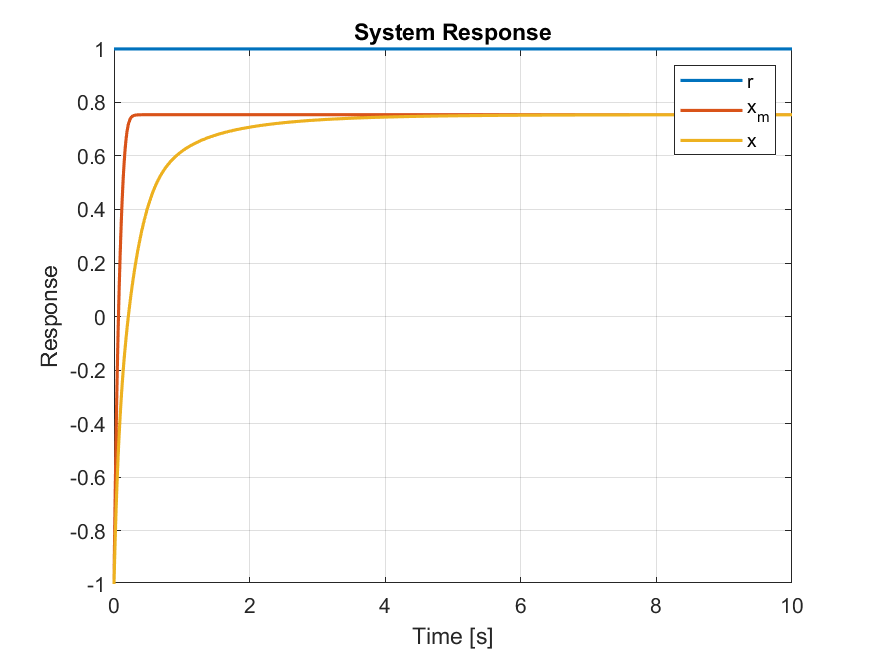
\includegraphics[width=\linewidth]{images/NL-MRAC-SIM/Step/v2/NMRAC_First-Order_Response.png}
  \caption{System response}
  \label{fig:step}
 \end{subfigure}
 \hfill
 \begin{subfigure}[b]{0.49\linewidth}
  \centering
  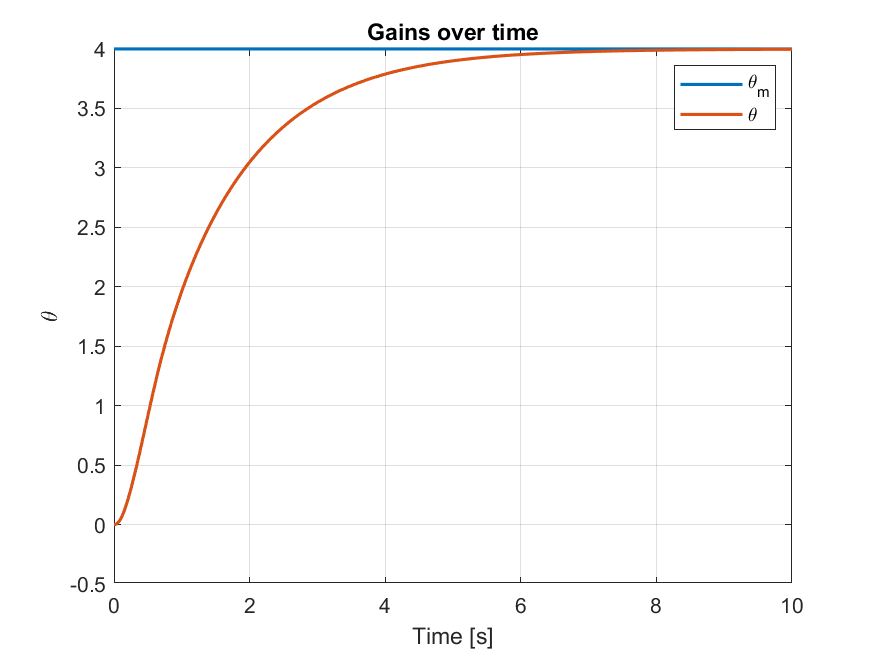
\includegraphics[width=\linewidth]{images/NL-MRAC-SIM/Step/v2/NMRAC_First-Order_Parameters.png}
  \caption{Evolution of the updated gain}
  \label{fig:step-weights}
 \end{subfigure}
 \caption{Simulation results of nonlinear MRAC with a constant input}
 \label{fig:nl-step}
\end{figure}


\begin{figure}[!t]
 \centering
 \begin{subfigure}[b]{0.49\linewidth}
  \centering
  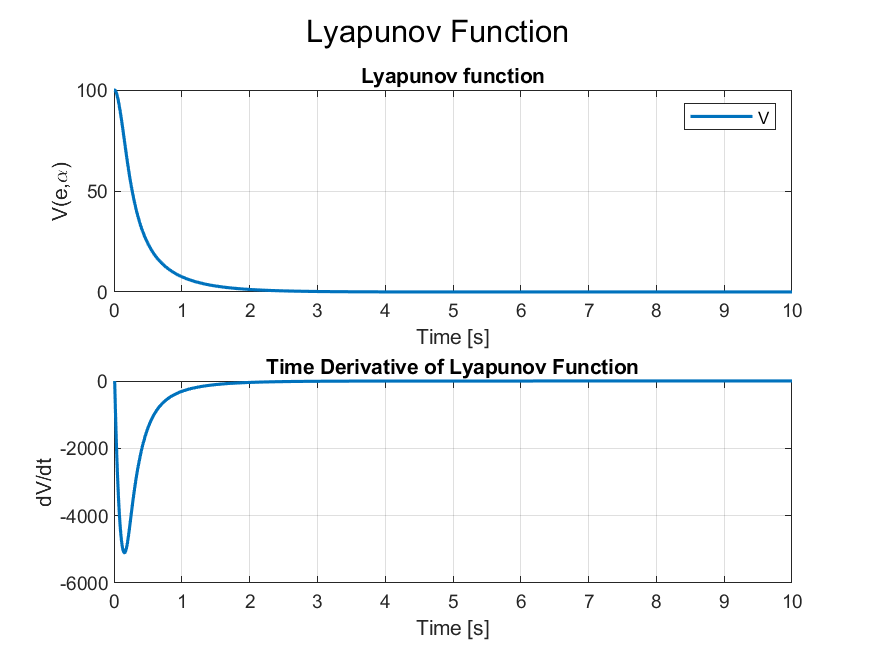
\includegraphics[width=\linewidth]{images/NL-MRAC-SIM/Step/v2/NMRAC_First-Order_Lyapunov.png}
  \caption{Lyapunov function and its time derivate}
  \label{fig:Lyapunov-step-input}
 \end{subfigure}
 \hfill
 \begin{subfigure}[b]{0.49\linewidth}
  \centering
  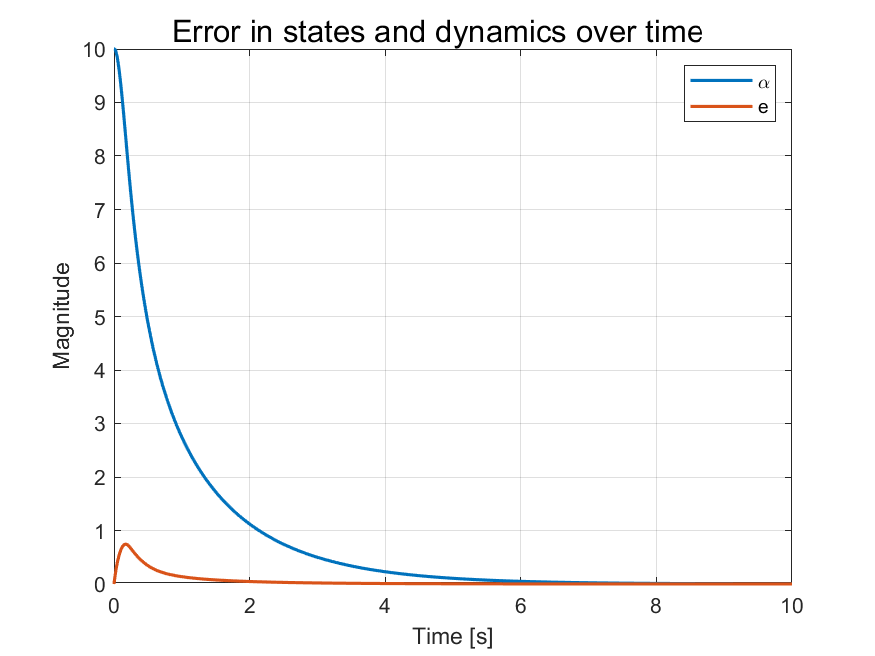
\includegraphics[width=\linewidth]{images/NL-MRAC-SIM/Step/v2/NMRAC_First-Order_Alpha.png}
  \caption{Error in internal states and dynamics of the system}
  \label{fig:step-error}
 \end{subfigure}
 \caption{Lyapunov function and convergence of the system w.r.t. internal states and dynamics}
 \label{fig:step-lyap}
\end{figure}

\subsection{Sine Signal}
\label{sec:sine}
The second reference is a sinusoidal signal, with an amplitude of $0.25$, to stay in a region that is not too heavily affected by the saturation of the controller. Again, the initial $\theta$ and $\theta_m$ are chosen to be $0$ and $4$, respectively. The initial conditions of both the system and the model reference are at $x=x_m=-1$. Finally, the system response is simulated for $30$ seconds and the learning rate is chosen to be $c=0.15$, which corresponds to a less aggressive learning strategy compared to the case of the constant input signal.

Fig. \ref{fig:sine} shows the response of the system. It can be observed that the system state and the model reference state both converge in around $25$ seconds. Simultaneously, the parameter $\theta$ converges towards the desired value $\theta_m = 4$, as shown in Fig. \ref{fig:sine-weights}. Even though the parameter converges, oscillations can be observed. This behavior is expected, due to the update law. Since the update law is dependent on $\dot e_x$, it is dependent on $\dot r$ and $\dot x$. Whenever $\dot e_x$ switches signs and simultaneously $e$ is small, $\dot \theta$ changes sign, and hence the parameter starts oscillating. This behavior can be influenced by adapting the learning rate. A more aggressive learning strategy will be showcased in the next example.

In Fig. \ref{fig:Lyapunov-sine-input} the Lyapunov function is shown, which converges to zero over time. Additionally, the time derivative of the Lyapunov function is negative and only reaches zero when the Lyapunov function itself converges to zero. Again, the results of this simulation indicate that the proposed learning algorithm is stable for the desired reference signal.

\begin{figure}[!t]
 \centering
 \begin{subfigure}[b]{0.49\linewidth}
  \centering
  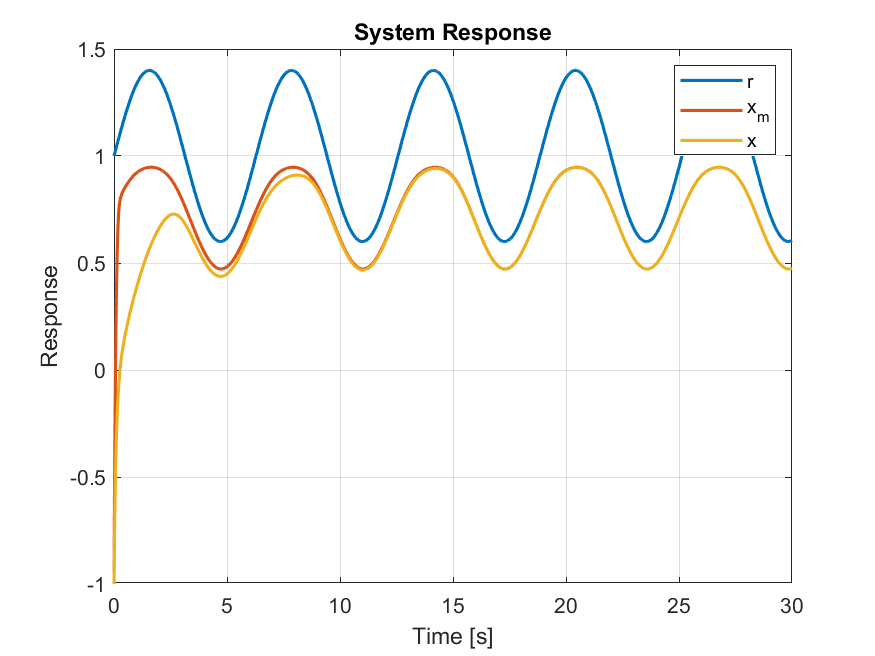
\includegraphics[width=\linewidth]{images/NL-MRAC-SIM/Sine/v2/NMRAC_First-Order_Response.png}
  \caption{System response}
  \label{fig:sine}
 \end{subfigure}
 \hfill
 \begin{subfigure}[b]{0.49\linewidth}
  \centering
  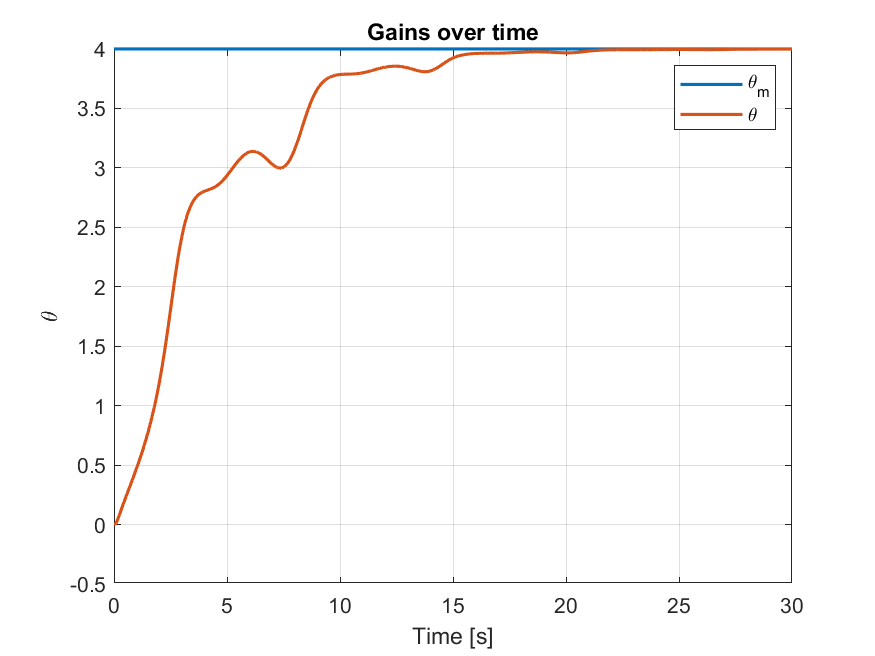
\includegraphics[width=\linewidth]{images/NL-MRAC-SIM/Sine/v2/NMRAC_First-Order_Parameters.png}
  \caption{Evolution of the updated gain}
  \label{fig:sine-weights}
 \end{subfigure}
 \caption{Simulation results of nonlinear MRAC with a sine input}
 \label{fig:nl-sine}
\end{figure}


\begin{figure}[!t]
 \centering
 \begin{subfigure}[b]{0.49\linewidth}
  \centering
  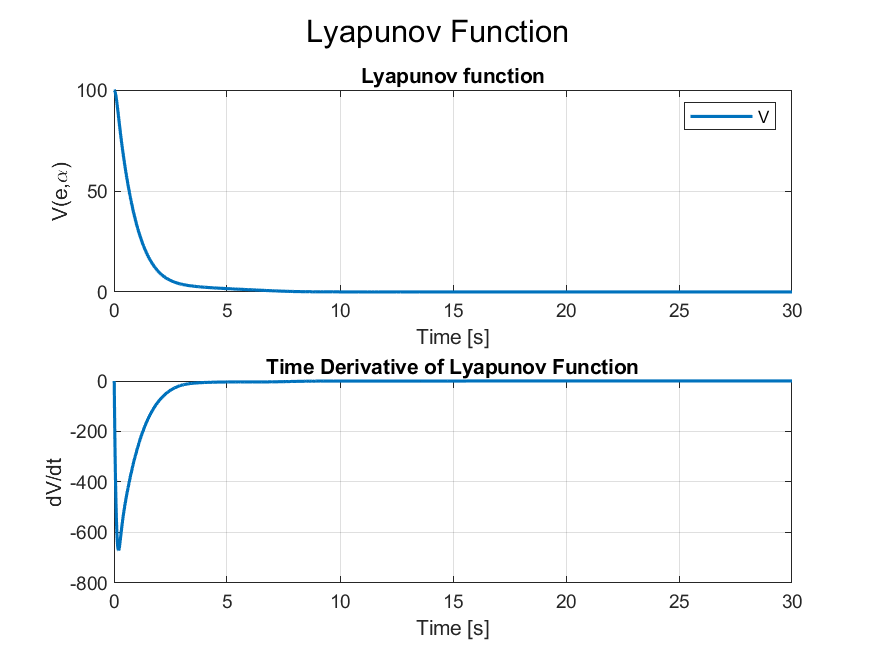
\includegraphics[width=\linewidth]{images/NL-MRAC-SIM/Sine/v2/NMRAC_First-Order_Lyapunov.png}
  \caption{Lyapunov function and its time derivate}
  \label{fig:Lyapunov-sine-input}
 \end{subfigure}
 \hfill
 \begin{subfigure}[b]{0.49\linewidth}
  \centering
  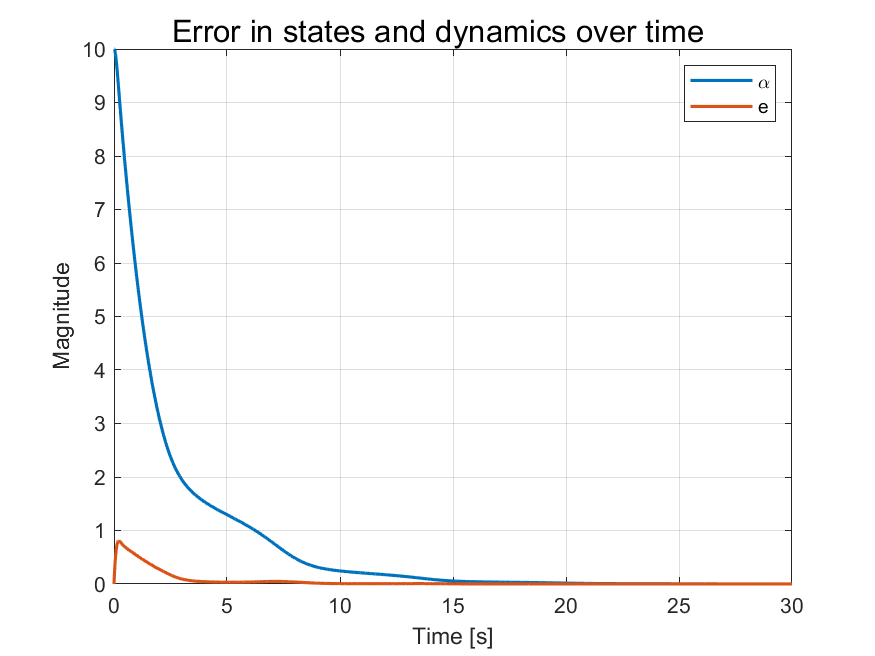
\includegraphics[width=\linewidth]{images/NL-MRAC-SIM/Sine/v2/NMRAC_First-Order_Alpha.png}
  \caption{Error in internal states and dynamics of the system}
  \label{fig:error}
 \end{subfigure}
 \caption{Lyapunov function and convergence of the system w.r.t. internal states and dynamics}
 \label{fig:lyap}
\end{figure}


\subsection{Smooth Pulse Signal}
The third and last input signal is a pulse signal. More specifically, a smooth pulse signal is used, since the update law requires a continuous time derivative of the reference signal. The smooth pulse signal is constructed, by using a sine function and applying a smooth saturation function, as defined in \eqref{eq:sigmoid}. The signal is chosen to have an amplitude of $0.25$ and a bias such that its minimum value touches upon $0$. As before, the initial conditions of the system and plant are $x=x_m=-1$. The response is simulated for $5$ seconds and a learning rate of $c=0.005$ is chosen.

Fig. \ref{fig:pulse} shows the response of the system. It can be observed that the system converges towards the model reference within just under $1$ second. The parameter $\theta$ converges towards the desired value within $2$ seconds, as shown in Fig. \ref{fig:pulse-weights}. Even though the parameter converges, there are oscillations present. They are present due to the same argument as for the sine signal, as explained in Section \ref{sec:sine}.

The Lyapunov function and its derivative, as shown in Fig. \ref{fig:Lyapunov-pulse-input} indicate the convergence of the system and the parameters, since $V$ converges to $0$ and its time derivative is always negative and converges to zero as well.

\begin{figure}[!t]
 \centering
 \begin{subfigure}[b]{0.49\linewidth}
  \centering
  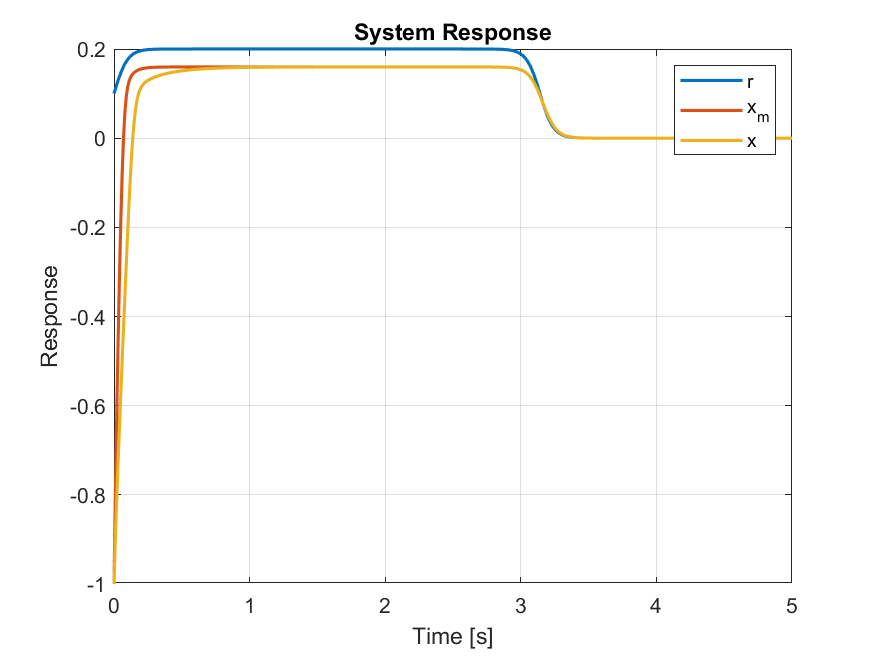
\includegraphics[width=\linewidth]{images/NL-MRAC-SIM/Smooth-Pulse/v2/NMRAC_First-Order_Response.png}
  \caption{System response}
  \label{fig:pulse}
 \end{subfigure}
 \hfill
 \begin{subfigure}[b]{0.49\linewidth}
  \centering
  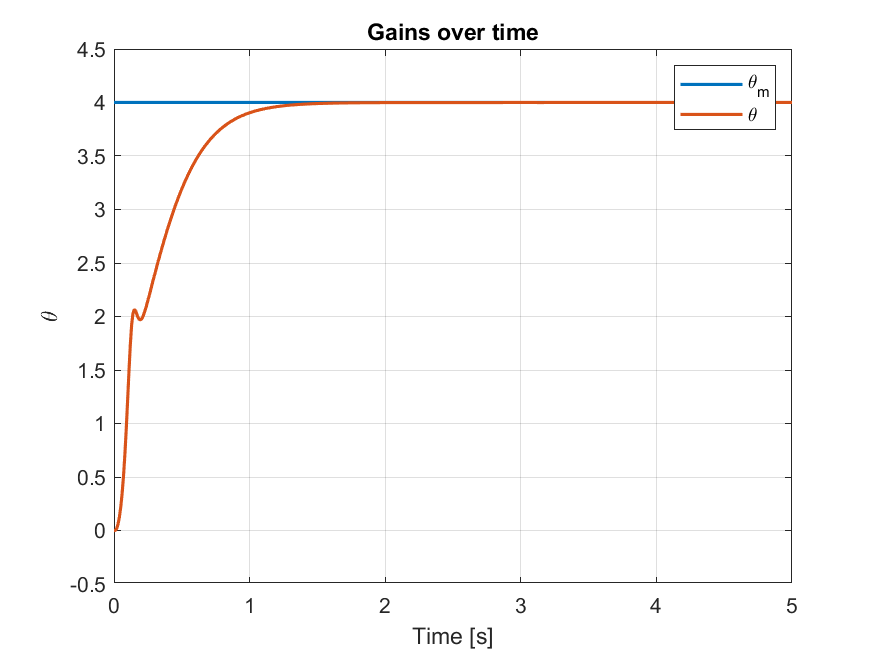
\includegraphics[width=\linewidth]{images/NL-MRAC-SIM/Smooth-Pulse/v2/NMRAC_First-Order_Parameters.png}
  \caption{Evolution of the updated gain}
  \label{fig:pulse-weights}
 \end{subfigure}
 \caption{Simulation results of nonlinear MRAC with a smooth pulse input}
 \label{fig:nl-pulse}
\end{figure}


\begin{figure}[!t]
 \centering
 \begin{subfigure}[b]{0.49\linewidth}
  \centering
  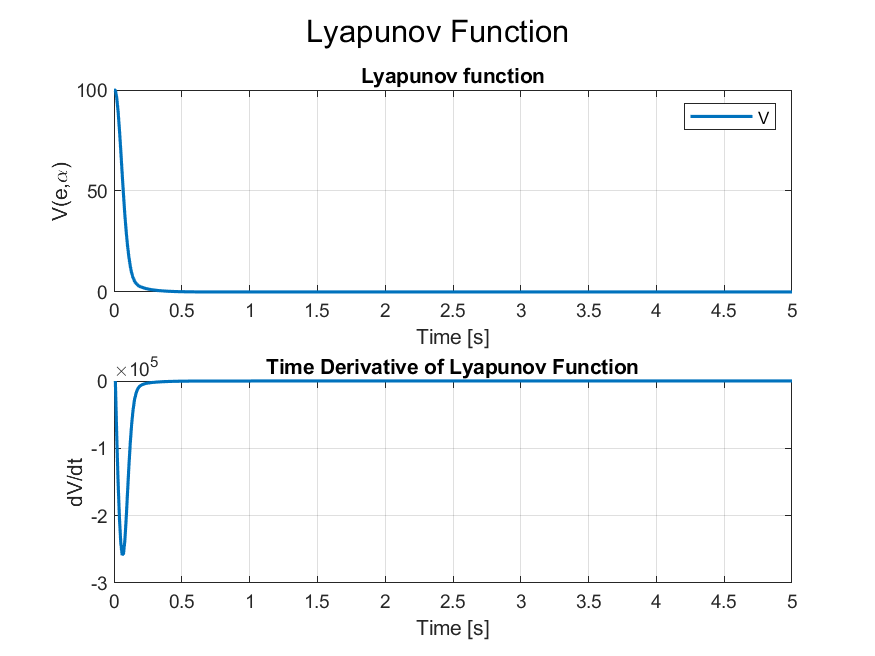
\includegraphics[width=\linewidth]{images/NL-MRAC-SIM/Smooth-Pulse/v2/NMRAC_First-Order_Lyapunov.png}
  \caption{Lyapunov function and its time derivate}
  \label{fig:Lyapunov-pulse-input}
 \end{subfigure}
 \hfill
 \begin{subfigure}[b]{0.49\linewidth}
  \centering
  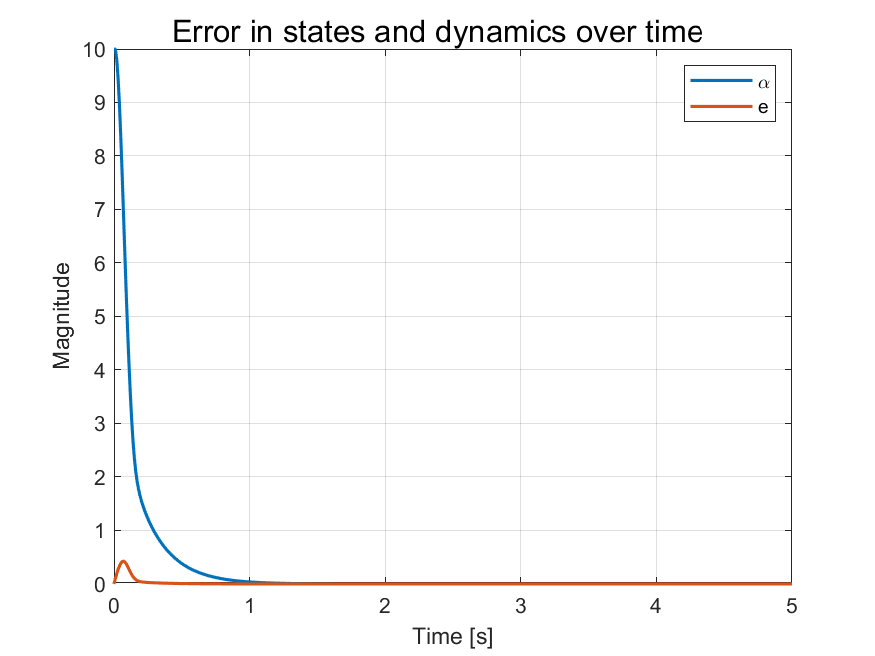
\includegraphics[width=\linewidth]{images/NL-MRAC-SIM/Smooth-Pulse/v2/NMRAC_First-Order_Alpha.png}
  \caption{Error in internal states and dynamics of the system}
  \label{fig:pulse-error}
 \end{subfigure}
 \caption{Lyapunov function and convergence of the system w.r.t. internal states and dynamics}
 \label{fig:pulse-lyap}
\end{figure}